% command line to generate Word docx
% pandoc -s "GAE723 - Travail 4.3 Comptes-rendus des suivis individuels - Vincent Le Falher - v1.0.tex" -o "GAE723 - Travail 4.3 Comptes-rendus des suivis individuels - Vincent Le Falher - v1.0.tex.docx"
\documentclass[12pt, letterpaper]{article}
\usepackage[utf8]{inputenc}
\usepackage{graphicx}
\usepackage[french]{babel}
\usepackage{todonotes}
\usepackage{comment} 
\usepackage{times}
\usepackage[T1]{fontenc} 
\usepackage[margin=2.54cm]{geometry}
\usepackage{colortbl}
\usepackage{color}
\usepackage[nottoc,numbib]{tocbibind}
\usepackage{flafter} % to force the table to be within it's section 
\usepackage[backend=biber]{biblatex}
\usepackage{lscape}
\usepackage{longtable}
\usepackage{draftwatermark}
\addbibresource{selection.bib}
\definecolor{orange}{rgb}{1,0.647,0}
\graphicspath{ {images/} }
\addto\captionsfrench{ \renewcommand*\contentsname{Table des matières} }
\addto\captionsfrench{ \renewcommand{\listfigurename}{Liste des figures} }
\addto\captionsfrench{ \renewcommand{\listtablename}{Liste des tableaux} }
\addto\captionsfrench{ \renewcommand{\bibname}{Références}}
\newcommand{\myparagraph}[1]{\paragraph{#1}\mbox{}\\\par}
\renewcommand{\tocbibname}{Bibliographie\label{chap:bib}}
\begin{document}
\begin{titlepage} % Suppresses headers and footers on the title page
   \centering % Centre everything on the title page
 
   \scshape % Use small caps for all text on the title page
  
   DÉPARTEMENT DE GÉOMATIQUE APPLIQUÉE\\Faculté des lettres et sciences humaines\\Université de Sherbrooke
   
   \vspace{10\baselineskip}
 
   {\LARGE Essai}
   \vspace{1\baselineskip}
   \linebreak
   {\LARGE Segmentation sémantique en temps réel à partir d'un nano-ordinateur: étude des performances et des limites.}
   \vspace{1\baselineskip}
   \linebreak
   \underline{{\LARGE Sous-titre}}
 
   \vspace*{3\baselineskip}
 
   \textit{Dans cadre de la maîtrise en sciences géographiques cheminement de type cours en géo développement durable}
   
   \vspace{5\baselineskip}
    
   VINCENT LE FALHER\\LEFV2603
     
   \vfill % Whitespace between editor names and year
 
   Longueuil\\Septembre 2020 % Publication year
 
\end{titlepage}
%----------------------------------------------------------------------------------------
\thispagestyle{empty}
\tableofcontents{}
\listoffigures{}
\listoftables{}
\newpage
\pagenumbering{arabic}
\section{Mise en contexte}
\noindent La compagnie \acrlong{pjcci} (\acrshort{pjcci}) désire évaluer la mise en service de la piste multifonctionnelle (vélos, piétons, etc.) du pont Jacques-Cartier, à Montréal, durant l'hiver. Pour ce faire, la piste doit rester sécuritaire et dégagée, malgré les évènements météorologiques.
\vspace{\baselineskip}
\\
\noindent L'Université de Sherbrooke, qui participe à cette initiative, propose de mettre en place sur le pont une plateforme de détection innovatrice qui consiste à installer plusieurs paires d'objets connectés ultralégers et performants (des nano ordinateurs) à différents endroits du pont. Chacun de ces nano ordinateurs possède trois différents types de capteurs: vision; son; et météorologiques (température, humidité, etc.). Chaque nano ordinateur d'une paire perçoit le même environnement, mais d'une perspective différente que son homologue: la caméra pointe vers la même surface, mais d'un autre point de vue; les sons et les données météorologiques sont captés dans le même voisinage. Les données collectées par les capteurs sont traitées en temps réel par des algorithmes de segmentation qui sont adaptés à ce type de problématiques : les réseaux de neurones, du domaine de l'intelligence artificielle. La déduction de l'état de la surface de la piste (sèche, mouillée, glacée, etc.) se fait en fusionnant les différentes perceptions (multicibles) de chaque capteur (multicapteurs).
\vspace{\baselineskip}
\\
\noindent Cet essai se concentre sur le volet vision du projet pour \acrshort{pjcci}. Il s'agit de déployer rapidement, facilement, et en grande quantité \todo{environs ? 25 ?} des nano ordinateurs tout le long de la piste multifonctionnelle du pont. Lors de la mise en service des nano ordinateurs, leur caméra sera simplement orientée vers la piste multifonctionnelle, et le modèle \acrshort{ia} devra détecter automatiquement dès son exécution (inférence), et d'une façon continue (opérationnalisation 24/7), les délimitations (segmentation) de la piste, sans avoir à lui fournir des paramètres ou réglages personnalisés, tels que l'angle de vue, la distance ou la hauteur. Les délimitations de la piste pourront ensuite être transmises à un autre programme installé sur le nano ordinateur afin de détecter en temps réel ou semi-temps réel\footnote{Temps réel signifie qu'il n'y a pas de délai entre le traitement de la donnée, et la communication du résultat. Semi-temps réel signifie qu'un faible délai est permis entre l'occurrence de l'évènement et la communication du résultat.}, les conditions de la surface de la piste multifonctionnelle: enneigée, mouillée, présence de glace noire, partiellement sèche, etc. Les résultats de la détection seront accessibles ou transmit via un accès à distance aux responsables de \acrshort{pjcci} afin qu'ils puissent prendre les décisions adéquates en matière d'entretien et d'accès. 
\vspace{\baselineskip}
\\
\noindent La détection d'objets en temps réel est de plus en plus précise et efficace depuis que les performances des systèmes informatisés permettent l'exécution d'algorithmes exigeants, en majeure partie depuis l'utilisation des processeurs graphiques "\acrshort{gpu}" \parencite{chong_real-time_1992, dettmers_deep_2015, beam_deep_2017, jiaconda_concise_2019, zheng_real-time_2020, kurenkov_brief_2015}. 
\vspace{\baselineskip}
\\
\noindent Les nano ordinateurs et les objets connectés, désignés aussi par l'"\acrlong{iot}" ou "\acrshort{iot}", \parencite{blanco-filgueira_deep_2019, sharma_history_2019} sont le résultat de la miniaturisation des systèmes informatiques. Ils permettent la détection en temps réel à des endroits, dans des situations et dans des conditions qui n'étaient pas envisageables il y a encore 10 ans \parencite{zheng_real-time_2020, bernas_edge_2017, abouzahir_iot-empowered_2017, blanco-filgueira_deep_2019}.
\vspace{\baselineskip}
\\
\noindent Les réseaux de neurones ont aussi rapidement progressé depuis 2012 \parencite{beam_deep_2017}, permettant d'offrir des alternatives aux solutions de détection et de classifications tel que les algorithmes SIFT et HOG \parencite{pathak_architecturally_2019}. Les réseaux de neurones pleinement connectés ("\acrshort{fcn}" en anglais, pour "\acrlong{fcn}") sont les derniers à avoir émergé et représente l'état de l'art (en anglais "state-of-art") \parencite{zheng_real-time_2020} et à profiter au domaine de la vision et de la détection d'objets \parencite{nguyen_mavnet_2019, zheng_real-time_2020}.
\vspace{\baselineskip}
\\
\noindent La segmentation sémantique est une forme de classification d'image, pixel par pixel, qui tire profit des dernières évolutions de la classification supervisée grâce aux réseaux de neurones pleinement connectés (\acrshort{fcn}), et qui peut être réalisée en temps réel avec des nano ordinateurs \parencite{long_fully_2015, blanco-filgueira_deep_2019}. Les images doivent être de haute résolution, ce qui nécessite d'avoir à disposition un système informatique capable de fournir une puissance de calcul appropriée, particulièrement pour la manipulation de la mémoire et des nombres flottants pendant l'inférence \parencite{mody_low_2018}. Leur application par des nano ordinateurs est un défi en raison de la faible consommation d'énergie (Watts) et de la puissance de calcul limité de ces derniers \parencite{copel_whats_2016}.
\vspace{\baselineskip}
\\
\noindent Pour \acrshort{pjcci}, les avantages d'une telle plateforme seraient multiples, et on peut en énumérer plusieurs, sans se limiter à: contrôler et mesurer l'épandage de sel; surveiller à distance les conditions de la piste multifonctionnelle; éviter le déplacement d'un spécialiste; suivre les effets du gel et du dégel; optimiser les couts des opérations d'entretien (déplacements, quantité); offrir aux usagers des conditions d'accès sécurisées et optimales même en hiver; effets environnementaux atténués; prise de décision et gestion proactive; planification.
\vspace{\baselineskip}
\\
\noindent D'un autre côté, les défis ne sont pas à sous-évaluer: la détection doit être précise, fiable et consistante, tout cela afin d'assurer aux usagers un service de qualité dans un contexte sécuritaire.
\section{Problématique}
\noindent Dans le cadre du projet pour \acrshort{pjcci}, une plateforme technologique sera mise à la disposition des gestionnaires du pont afin de les aider à prendre les décisions les plus responsables et raisonnables possibles. Mais la mise en service d'une solution innovante et fiable, qui concilie des algorithmes d'apprentissage profond, du temps réel, des nano-ordinateurs, et des conditions climatiques variables, est complexe. Dans une certaine mesure, l'essai va contribuer à la recherche de solutions afin de répondre au défi pour le domaine du transport actif et durable d'être soutenu par des solutions technologiques fiables (opérationnelles), l'objectif étant de pouvoir offrir des services de qualité et sécuritaires sur l'ensemble des quatre saisons.
\begin{comment}
\vspace{0.5\baselineskip}
\\
\noindent Il est difficile de trouver des jeux de données pour entrainer les réseaux de neurones pleinement connectés (\acrshort{fcn}) adaptés à la problématique. La technique de transfert d'apprentissage permet de démarrer d'une architecture qui a déjà appris avec un jeu d'images important (milliers d'images), et de lui faire apprendre davantage, en lui fournissant un plus petit jeu d'images (centaines d'images) de la nouvelle zone d'étude. Par exemple une architecture peut avoir appris à classifier des images de la Californie, aux États-Unis. Pour lui permettre de classifier des images de la Ville de Sherbrooke, il est souhaitable de lui fournir un nouveau jeu de données spécifique à cette ville afin qu'il s'adapte (ses paramètres) à cette région. Dans le contexte de cet essai, cela se traduit par réentrainer différents modèles avec des images de la piste multifonctionnelle du pont Jacques-Cartier.
\end{comment}
\vspace{0.5\baselineskip}
\\
\noindent La paramétrisation (des "hyper-paramètres") des réseaux de neurones est subtile et intuitive, et requière de l'expérience. C'est un processus d'essais-erreurs qui est couteux en temps, et risqué puisqu'il n'y a aucune garantie de succès. La technique d'apprentissage par transfert ("Transfer Learning" en anglais) permet d'hériter d'une architecture qui est déjà entrainée et paramétrée, et de l'adapter à d'autres problématiques, en lui fournissant un plus petit jeu d'images (une centaine) de la nouvelle zone d'étude. Cette technique permet un gain en temps puisque la phase de conception (analyse, architecture, configuration) est raccourcie de façon importante.
\begin{comment}
Par exemple l'architecture "VGG" prend 2-3 semaines d'entrainement \parencite{simonyan_very_2015} avec 4 \acrshort{gpu} Titan Black (NVIDIA), coutant 1 200 \$US (Amazon.com) chacun (pour un total de 4 800\$US, et cela juste pour les \acrshort{gpu}s, qui ne sont qu'un des éléments de l'infrastructure nécessaire). Étant donné que de multiples tentatives sont nécessaires (cycles essai-erreur), la stratégie est d'entrainer plusieurs modèles en parallèle afin d'accélérer le développement, ce qui implique un cout élevé en infrastructure.
\end{comment}
La problématique pour l'essai est de trouver l'architecture qui est la plus adaptée pour répondre au besoin, et il en existe des milliers \parencite{koh_model_2018}. La recherche dans la littérature permet heureusement de limiter les choix et donner des pistes \parencite{zheng_real-time_2020, nguyen_mavnet_2019, nvidia_jetson_2019-1}. 
\vspace{0.5\baselineskip}
\\
\noindent Même si les scores sont satisfaisants lors de la phase de test du modèle, la réalité du terrain peut surprendre. Les tests d'acceptation du modèle doivent se faire en dehors de l'environnement d'entrainement (laboratoire), dans les conditions réelles (luminosité, angle, hauteur, etc.) sur le terrain d'implémentation. Dans le jargon de l'intelligence artificielle et des réseaux de neurones, c'est l'inférence\footnote{Le terme "inférence" est utilisé lorsqu'un modèle, entrainé avec un échantillon de la population, est appliqué pour pouvoir donner une conclusion pour d'autres échantillons de la population (déduire un chien ou un chat sur une image). Le terme "prédiction" est utilisé lorsqu'un modèle, entrainé avec un échantillon de la population, est appliqué pour déduire une valeur selon une ou plusieurs variables (la température selon la localisation et l'altitude).} \parencite{copel_whats_2016, nvidia_jetson_2019-1}. De plus, le système hôte, dans notre cas le nano-ordinateur NVIDIA Jetson Nano, est conçu avec une architecture matérielle limitée (\acrshort{gpu}, \acrshort{cpu}s, mémoire, taux de transfert, alimentation). 
\vspace{0.5\baselineskip}
\\
\noindent La segmentation sémantique (figure \ref{fig:semantic_segmentation_vs_others}) est une forme de classification d'image, pixel par pixel, qui tire profit des dernières évolutions de la classification supervisée grâce aux réseaux de neurones pleinement connectés (\acrshort{fcn}), et qui peut être réalisée en temps réel avec des nano-ordinateurs \parencite{long_fully_2015, blanco-filgueira_deep_2019}. Les images doivent être de haute résolution, ce qui nécessite d'avoir à disposition un système informatique capable de fournir une puissance de calcul appropriée, particulièrement pour la manipulation de la mémoire et des nombres flottants pendant l'inférence \parencite{mody_low_2018}. Leur application par des nano-ordinateurs est un défi en raison de la faible consommation d'énergie (Watts) et de la puissance de calcul limité de ces derniers \parencite{copel_whats_2016}.
\begin{figure}[H]
    \centering
    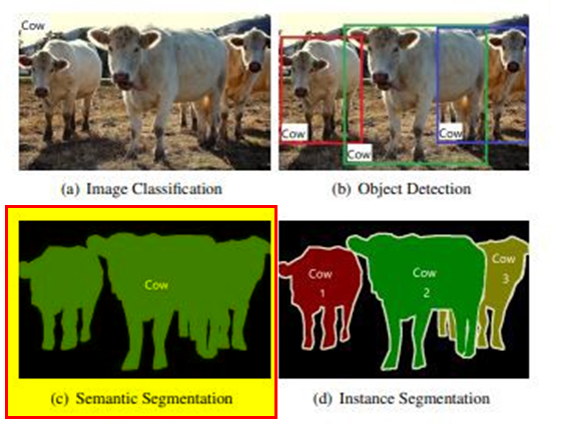
\includegraphics[width=0.75\textwidth]{semantic_segmentation_vs_others}
    \caption[Segmentation semantic]{Segmentation semantic\parencite[p.~1]{wu_recent_2019}}
    \label{fig:semantic_segmentation_vs_others}
 \end{figure}
\noindent Il existe différents cadres applicatifs pour l'entrainement de modèles \acrshort{ia}, tels que PyTorch ou TensorFlow. L'inconvénient est d'avoir à installer pour chacun leur propre environnement de développement et d'inférence, ce qui augmente les efforts et les coûts. Le cadre applicatif ONNX a été conçu pour pallier cette contrainte. En effet, il uniformise les architectures des modèles, et simplifie la mise en service grâce à l'installation d'un unique cadre applicatif. NVIDIA fournit avec le Jetson Nano une plateforme applicative qui supporte les modèles convertis au format ONNX, et offre donc une solution supportant l'interopérationabilité des modèles \acrshort{ia}. 
\section{Objectifs}
\noindent L'objectif principal de cet essai consiste a étudier la capacité du nano ordinateur du fabricant NVIDIA, le Jetson Nano \parencite{nvidia_jetson_2019}, à exécuter, en temps réel, une architecture de réseau de neurones pleinement connectés (\acrshort{fcnn}) entrainée à faire de la segmentation sémantique d'images et de vidéos de hautes résolutions qui sont perçues avec la caméra. Une seule classe sera extraite, celle représentant la piste multifonctionnelle. Les autres classes ne seront pas utilisées. Il semble important de préciser que l'objectif de l'essai n'est pas d'évaluer la précision (\acrshort{iou},  F1 score) de la segmentation sémantique, mais de déterminer, et ce en rapport avec les attentes du projet pour \acrshort{pjcci}, si la segmentation sémantique en temps réel d'une vidéo de haute qualité avec le Jetson Nano dans un mode opérationnel 24/7 est viable, et si les délimitations de la piste multifonctionnelle sont jugées acceptables pour être utilisée par un autre programme pour détecter les conditions de la surface.
\vspace{\baselineskip}
\\
\noindent Les sous-objectifs sont les suivants: 
\begin{itemize}
   \item Évaluer les limites de la plateforme, matérielle et applicative.
   \item Évaluer les moyens d'optimiser la plateforme d'un point de vue matériel et applicatif. 
   \item Évaluer la possibilité de pouvoir ré entrainer l'architecture sur le nano ordinateur dans une perspective d'apprentissage actif et continue.
   \item Ré entrainer une architecture \acrshort{fcnn} avec les images du site d'implémentation.
   \item Permettre un accès à distance sécurisé au nano ordinateur.
   \item Documenter l'approche, les tests, et les résultats;
\end{itemize}
\vspace{\baselineskip}
\noindent Il n'est pas planifier de faire des tests sur le site d'implémentation, ni s'intégrer avec d'autres programmes du projet pour \acrshort{pjcci}, par exemple pour détecter les conditions de la surface de la piste multifonctionnelle. 
\vspace{\baselineskip}
\\
\noindent Le premier sous-objectif est de déterminer quelles sont les limites de la plateforme, d'un point de vue matériel (\acrshort{gpu}, \acrshort{cpu}s, mémoire, transfert mémoire, consommation, etc.), mais aussi applicatif, d'un point de vue inférence. Cette phase du projet va permettre d'exécuter tel quel différents modèles d'architecture déjà existants, sans les ré entrainer, en tenant compte des éléments documentés dans la littérature \parencite{nguyen_mavnet_2019, zheng_real-time_2020, nvidia_jetson_2019-1}.
\vspace{\baselineskip}
\\
\noindent Un autre sous-objectif est d'optimiser ou d'adapter la plateforme, d'un point de vue matériel, mais aussi applicatif, afin d'avoir les meilleures performances et résultats possibles pendant l'inférence.
\vspace{\baselineskip}
\\
\noindent L'un des intérêts de l'\acrshort{ia} est de pouvoir améliorer constamment les modèles grâce au ré entrainment continue. L'essai va évaluer la possibilité de bénéficier de cet avantage directement sur le nano ordinateur en tentant de ré entrainer activement l'architecture avec des images de la piste multifonctionnelle re segmentées par un expert, et re générer un modèle plus précis, tout ceci en concurence avec l'inférence en temps réel. 
\vspace{\baselineskip}
\\
\noindent Comme les résultats devront être disponibles en tout temps, une connexion à distance sécurisée devra être mise en place. Cette connexion permettra aussi de pouvoir prendre le contrôle du nano ordinateur à distance et de l'administrer. En effet, le nano ordinateur sera déployé sur le site d'implémentation sans les périphériques standards, tel qu'un clavier, souris ou écran. Le type de réseau adéquat, soit Ethernet ou cellulaire (carte SIM réseau 3g/4g), sera évalué.
\vspace{\baselineskip}
\\
\noindent L'approche, les tests, et les résultats sont documentés. Il y aura beaucoup d'activités relatives à la conception et aux tests, le cheminement complet n'est pas fourni. Une synthèse est préférée et les informations les plus pertinentes sont incluses. Les détails de l'installation de l'environnement de développement et des applications, librairies et autres dépendances nécessaires sont inclus, ainsi que ceux de la configuration. Dans le cas où l'objectif principal n'est pas atteint, ou partiellement, la/les raison/s de l'échec sont spécifiées et des pistes de solutions potentielles proposées.
\section{Identification des besoins en termes de données}
Voici les données qui ont été identifiées comme nécessaires.
\begin{itemize}
   \item jeux de données (images) d'entrainement des modèles existants;
   \item vidéos de la zone d'étude; 
   \item nouvelles images, extraites des vidéos;
\end{itemize}
\vspace{1\baselineskip}
\par Il existe déjà des modèles de réseaux de neurones dont l'application est la segmentation sémantique. Ces modèles ont été entraînés avec des jeux de données qui sont disponibles gratuitement. Il est planifié utiliser ces modèles déjà pré-entrainés, et les ré-entrainer en bonifiant les jeux de données d'entrainement avec des données locales. Ces jeux de données seront aussi utiles pour valider et tester le résultat du ré-entrainement.
\par Selon nos recherches, à ce jour, il n'existe pas de modèles de réseaux de neurones qui ont été entrainés pour répondre directement aux objectifs de l'essai. Il sera donc nécessaire de construire des jeux de données représentant la zone d'étude, le "nouveau domaine" de l'apprentissage. Ces nouvelles images permettront d'adapter à ce nouveau domaine les modèles de réseaux de neurones qui auront été sélectionnés (technique "Adaptation domain" en anglais). Les images seront extraites des vidéos acquises dans les conditions décrites ci-après (section \ref{sect:conditions}).
\par Les vidéos sont la source de données principales de l'essai: l'inférence est faite à partir de vidéos en temps réel. La résolution et le nombre d'images par seconde seront à déterminer. Les vidéos seront acquises dans les conditions décrites ci-après (section \ref{sect:conditions}).

\subsection{Stratégie de recherche de données}
Voici les stratégies qui ont été identifiées pour la recherche de données.
\begin{itemize}
   \item resources NVIDIA;
   \item références en lien avec le sujet;
   \item Internet;
   \item Association des piétons et cyclistes du pont Jacques-Cartier;
   \item travaux d'étudiants de l'Université de Sherbrooke;
   \item acquisition des vidéos de la piste multifonctionnelle du pont Jacques-Cartier;
   \item discussions avec mon directeur de projet;
\end{itemize}
\vspace{1\baselineskip}
\par Les ressources mises à disposition par le constructeur du Jetson nano, NVIDIA, seront étudiées pour apprendre et tester le nano-ordinateur. Parmi les plus intéressantes, on peut citer le "Jetson Nano Developer Kit", le "NVIDIA Deep Learning Institute", la communauté Jetson, les tutoriels, les "benchmarks". Des jeux de données sont fournis gratuitement.
\par En complément des ressources de NVIDIA, deux références scientifiques seront principalement utilisées comme points de départ et comme modèles pour l'essai, car leurs études ont été faites avec le Jetson nano (\cite{nguyen_mavnet_2019} et \cite{chong_real-time_1992}). Beaucoup de références ont été publiées ces deux dernières années sur le sujet de la segmentation sémantique, ils existent donc de multiples alternatives inspirantes.
\par Internet est une mine d'information et de données. Il existe des forums et des blogues dans lesquels des utilisateurs publient leurs expérimentations de la segmentation sémantique en temps réel avec le Jetson nano (\cite{dustin_realtime_2019}), ou plus génériquement la segmentation sémantique. Des sites comme "modelzoo.co" sont des entrepôts de modèles déjà pré-entrainés. Une autre option est d'effectuer une recherche d'images ou de vidéos de la piste multifonctionnelle du pont Jacques-Cartier via les sites de recherche tels que Google. 
\par L'Association des piétons et cyclistes du pont Jacques-Cartier existe depuis de nombreuses années pour promouvoir le transport actif et conserver la piste multifonctionnelle du pont Jacques Cartier ouverte durant l'hiver. Ils fournissent, via des sites Internet, des collections de vidéos et d'images qui pourraient être utilisées. Il serait aussi possible d'entrer en contact avec l'association et leur demander de prendre de nouvelles vidéos. Voir http://pontjacquescartier365.com, et https://www.flickr.com/photos/pontjacquescartier.
\par Une autre possibilité serait d'hériter des acquisitions faites par un autre étudiant de l'université de Sherbrooke, soit déjà archivée, soit collectée prochainement. Mon directeur de projet Mickaël G. m'a informé qu'un étudiant de Sherbrooke va avoir besoin de collecter le trafic automobile sur le campus de l'Université de Sherbrooke, à Sherbrooke. 
\par Enfin il y a l'acquisition des vidéos spécifiquement pour le projet PJCCI, tel que documenté à la section \ref{sect:conditions}. Comme il n'y a aucune date de planifiée pour la capture des vidéos, l'essai devra s'arranger pour dépendre le moins possible d'elles durant la préparation et le développement, et s'attendre à les recevoir pour le ré-apprentissage et les tests, en fin d'essai.
\par Tout au long de l'essai, mon directeur Mickaël sera une ressource importante afin de vérifier que les sources de données, les prétraitements et les traitements sont adéquats aux attentes du projet pour PJCCI.

\subsection{Conditions d'acquisition des nouvelles données} \label{sect:conditions}
\par Les images et vidéos qui seront acquises devront répondre à différents requis, afin de pouvoir adapter le modèle de réseau de neurones dans des conditions les plus proches de la réalité. 
\begin{itemize}
   \item L'objet d'intérêt pour la collecte des données est la surface de la piste multifonctionnelle du pont Jacques-Cartier, à Montréal (Québec, Canada). 
   \item L'acquisition se fera à partir de différents points d'intérêt sur le pont. Ces points d'intérêt seront déterminés par les gestionnaires du projet pour PJCCI. 
   \item L'appareil d'acquisition sera installé sur un trépied pendant la capture afin d'avoir un point de vue stable et constant. 
   \item Pour chaque point d'intérêt, la hauteur du trépied, en plus de son géoréférencement, l'angle de vision et la direction seront documentés. Les points d'intérêt seront géoréférencés afin d'être représentés sur une carte. La précision du géoréférencement devra être assez précise pour que d'autres acquisitions puissent avoir lieu. De plus, au moins trois points de référence sur les bords de l'image devront être déterminés pour garder le même angle de vision et la direction à chaque acquisition. 
   \item La capture sera faite pendant une période assez prolongée, telle que des périodes de 15 ou 30 minutes. La période d'acquisition est à la discrétion des architectes applicatifs du projet pour PJCCI.
   \item La même surface sera capturée de différents angles en simultané avec deux appareils d'acquisition. Cela permettra d'avoir deux images de la même zone au même moment, mais d'une perspective différente.
   \item Comme indiqué précédemment, plusieurs points d'intérêts de la piste multifonctionnelle seront capturés, toujours de différents angles en simultané.
   \item L'acquisition sera faite de jour.
   \item La luminosité devra être bonne, normale. 
   \item L'acquisition dans des conditions spéciales est exclue, telle que la nuit, une luminosité ou une visibilité extrême, comme aucune, ou médiocre.
   \item Des images des différentes conditions de la surface seront acquises: sèche, partiellement mouillée, trempée, partiellement recouverte de neige, recouverte de neige, glace noire, "slush", etc. Cela devrait correspondre aux classes du projet avec PJCCI et non celles de l'essai. Il existe de nombreuses références à ce sujet, par exemple \cite{cheng_road_2019}, \cite{fu_risk-based_2017}, \cite{pan_winter_nodate}.
   \item Les vidéos devront capturer du trafic: piéton, vélo, coureur, poussette, groupe, chiens en laisse, etc. Cela va permettre d'entrainer le modèle lorsqu'il y a des obstacles sur la piste et tester la fiabilité de la segmentation sémantique. 
   \item Les vidéos seront acquises en différentes résolutions: haute (1080p/i), puis de plus en plus faible 760p/i, 576p/i, 480p/i, 360p/i. Cela va permettre de tester les performances avec une perte progressive de la qualité (nombre de pixels).
   \item Les vidéos seront acquises avec un nombre d'images par seconde différente (FPS, "Frames Per Second" en anglais): élevés (30FPS), puis de moins en moins rapide, 20FPS, 10FSP, 1FPS. Cela va permettre de tester les performances et déterminer le meilleur compromis entre résolutions et FPS.
   \item Il n'est pas important que l'appareil d'acquisition soit le même que celui qui sera utilisé pendant l'essai, car les images sont adaptées par l'environnement de développement ("framework" en anglais) d'apprentissage profond au moment du prétraitement de l'entrainement.
   \item Comme il y aura une quantité non négligeable de nouvelles données acquises, qui de plus sont des données multimédias de haute résolution, un espace de rangement ("storage" en anglais) suffisant et performant sera nécessaire. Une espace de sauvegarde est de plus indispensable pour conserver les données brutes, mais aussi les différentes versions dues aux traitements. Un espace dans le nuage ("cloud") est une option non négligeable, mais la décision est à la discrétion des architectes applicatifs du projet pour PJCCI.
   \item Une nomenclature pour le nom des répertoires et des fichiers vidéos sera déterminée, à la discrétion des architectes applicatifs du projet pour PJCCI. Les données utilisées pour l'essai seront gérées à ma discrétion (espace de rangement, copies de sauvegarde, nomenclature).
\end{itemize}

\subsection{Synthèse des données}
\par Voici le tableau de synthèse des données, incluant la référence avec leur réseaux de neurones.
{
   \clearpage 
   \newpage
   \begin{landscape}
   \newcounter{magicrownumbers}
   \newcommand\rownumber{\stepcounter{magicrownumbers}\arabic{magicrownumbers}}
   % \centering
   \vspace{0.3em} % Adjust the height of the space between caption and tabular
   \begin{longtable}[t]{@{}p{1em}|p{15em}p{35em}@{}} % p{15em}p{35em} with landscape
      \caption{Tableau des données}\label{tab:datasets}\\
      & \textbf{Spécification} & \textbf{Description}\\
      \hline
      \endfirsthead
      & \textbf{Spécification} & \textbf{Description}\\
      \hline
      \endhead
      \endfoot
      \endlastfoot
      \hline
      \rownumber & \begin{tabular}[t]{@{}p{15em}@{}}
         réseau: U-Net\\jeu de données: Membrane (origine isbi challenge)\\nombre d'images: 30\\résolution/s: 512x512
      \end{tabular} & \begin{tabular}[t]{@{}p{35em}@{}}
         C'est le jeu de données pour le réseau U-Net. Il est utilisé dans le benchmark de NVIDIA pour l'inférence avec le Jetson nano. Les images sont de type médicale.\\
         À noter que le framework "Keras" s'occupe de l'augmentation de données.\\
         https://github.com/zhixuhao/unet/tree/master/data/membrane\\
      \end{tabular}\\
      \hline
      \rownumber & \begin{tabular}[t]{@{}p{15em}@{}}
         réseau: SegNet\\jeu de données: CamVid\\vidéos: 10 minutes\\résolution/s: HD
      \end{tabular} & \begin{tabular}[t]{@{}p{35em}@{}}
         SegNet est un réseau qui a été créé pour la segmentation sémantique de vidéos. Il a été entrainé avec le jeu de données de CamVid, qui procurents des vidéos de la route avec la méme perspective que le conducteur du véhicule. Un modèle entrainé est disponible pour le Jetson nano.\\
         https://github.com/PengKiKi/camvid\\
      \end{tabular}\\
      \hline
      \rownumber & \begin{tabular}[t]{@{}p{15em}@{}}
         réseau: MFANet\\jeu de données: Cityscapes\\nombre d'images: 5000\\résolution/s: 1280x1024
      \end{tabular} & \begin{tabular}[t]{@{}p{35em}@{}}
         MFANet est un réseau qui a été créé en 2019 pour la segmentation sémantique sur des appareils tel que le Jetson nano. Il a été entrainé avec le jeu de données de Cityscapes, qui procurents des images de scènes urbaines. Différentes stratégies d'augmentation de données sont utilisées. Des tests ont été fait avec le Jetson nano.\\
         leejy@ustb.edu.cn\\
      \end{tabular}\\
      \hline
      \rownumber & \begin{tabular}[t]{@{}p{15em}@{}}
         réseau: MAVNet\\jeu de données: Penstock\\nombre d'images: 135\\résolution/s: 1280x1024
      \end{tabular} & \begin{tabular}[t]{@{}p{35em}@{}}
         C'est l'un des deux jeux de données pour le réseau MAVNet. Les images sont celles de "conduites forcées", des voies d'eau de régulation, et sont préparées pour la segmentation sémantique. Des tests ont été fait avec le Jetson nano.\\
         https://github.com/tynguyen/MAVNet/tree/master/data/TN\_penstock\\
      \end{tabular}\\
      \hline
      \rownumber & \begin{tabular}[t]{@{}p{15em}@{}}
         réseau: MAVNet\\jeu de données: Penstock\\nombre d'images: 135\\résolution/s: 1280x1024
      \end{tabular} & \begin{tabular}[t]{@{}p{35em}@{}}
         C'est l'un des deux jeux de données pour le réseau MAVNet. Les images sont celles de drones volant à l'intérieur d'un bâtiment, et préparées pour la segmentation sémantique. Des tests ont été fait avec le Jetson nano.\\
         https://github.com/tynguyen/MAVNet/tree/master/data/perch\_drone\\
      \end{tabular}\\
      \hline
      \rownumber & \begin{tabular}[t]{@{}p{15em}@{}}
         réseau: RESNet18\\jeu de données: Cityscapes\\nombre d'images: 25 000\\résolution/s: 360x720, 512x256, 1024x512, 2048x1024
      \end{tabular} & \begin{tabular}[t]{@{}p{35em}@{}}
         Cityscapes est un jeu de données qui fournit des images de rues spécifiquement destinées pour la segmentation sémantique. Il peut être utilisé par de nombreux réseaux. RESNet18 a été entrainé avec ce jeu et est disponible en diverses résolutions pour le Jetson Nano.\\
         https://github.com/tynguyen/MAVNet/tree/master/data/perch\_drone\\
      \end{tabular}\\
      \hline
      \rownumber & \begin{tabular}[t]{@{}p{15em}@{}}
         réseau: RESNet18\\jeu de données: DeepScenes\\nombre d'images: 15 000\\résolution/s: 576x320, 864x480 
      \end{tabular} & \begin{tabular}[t]{@{}p{35em}@{}}
         DeepScene propose un modèle et un jeu de données. Le modèle est entrainé avec différents jeux de données, comme Cityscpapes, SUN-RGBD, Synthia. Le jeu de données fournit des images de forêt, qui est destinée pour la segmentation sémantique. RESNet18 a été entrainé avec ce jeu et est disponible en deux  résolutions pour le Jetson Nano.\\
         http://deepscene.cs.uni-freiburg.de\\
      \end{tabular}\\
      \hline
      \rownumber & \begin{tabular}[t]{@{}p{15em}@{}}
         réseau: RESNet18\\jeu de données: Multi-Human\\nombre d'images: 25 043\\résolution/s: 512x320, 640x360
      \end{tabular} & \begin{tabular}[t]{@{}p{35em}@{}}
         Le jeu de données Multi-Human fournit des images contenant des humains, et qui est destinée pour la segmentation sémantique. RESNet18 a été entrainé avec ce jeu et est disponible en deux résolutions pour le Jetson Nano.\\
         https://lv-mhp.github.io/dataset\\
      \end{tabular}\\
      \hline
      \rownumber & \begin{tabular}[t]{@{}p{15em}@{}}
         réseau: RESNet18\\jeu de données: Pascal VOC\\nombre d'images: 11 530\\résolution/s: 320x320, 512x320 
      \end{tabular} & \begin{tabular}[t]{@{}p{35em}@{}}
         Le jeu de données Pascal VOC fournit des images de classes variées tel que des personnes, des animaux, des véhicules, et des objets classiques, et qui peut être utilisé pour la segmentation sémantique. RESNet18 a été entrainé avec ce jeu et est disponible en deux résolutions pour le Jetson Nano.\\
         http://host.robots.ox.ac.uk/pascal/VOC/voc2012/index.html\\
      \end{tabular}\\
      \hline
      \rownumber & \begin{tabular}[t]{@{}p{15em}@{}}
         réseau: RESNet18\\jeu de données: SUN RGB-D\\nombre d'images: 10 335\\résolution/s: 512x400, 640x512
      \end{tabular} & \begin{tabular}[t]{@{}p{35em}@{}}
         Le jeu de données SUN RGB-D fournit des images de scènes d'intérieur de maison, et qui est destiné pour la segmentation sémantique. RESNet18 a été entrainé avec ce jeu.\\
         https://synthia-dataset.net\\
      \end{tabular}\\
      \hline
      \rownumber & \begin{tabular}[t]{@{}p{15em}@{}}
         réseau: DeepScene\\jeu de données: Synthia\\nombre d'images: 220 000\\résolution/s: 1280x760
      \end{tabular} & \begin{tabular}[t]{@{}p{35em}@{}}
         Le jeu de données Synthia fournit des images (et vidéos) de scènes de rue comme celui de Cityscapes, et qui est destiné pour la segmentation sémantique. DeepScene a été entrainé avec ce jeu. Il n'a pas été testé avec le Jetson Nano.\\
         http://3dvision.princeton.edu/datasets.html\\
      \end{tabular}\\
      \hline
      \rownumber & \begin{tabular}[t]{@{}p{15em}@{}}
         jeu de données: Association des piétons et cyclistes pont Jacques-Cartier\\nombre d'images: 313\\résolution/s: variées
      \end{tabular} & \begin{tabular}[t]{@{}p{35em}@{}}
         L'Association des piétons et cyclistes du pont Jacques-Cartier a une collection d'images et de vidéos de la piste multifonctionnelle du pont Jacques-Cartier. Ce n'est pas un jeu de données qui est prêt à être utilisé pour l'apprentissage tel-quel, il doit être préparé. Mais c'est une source de données qui est très importante pour l'essai. Il est envisagé de contacter l'association au besoin afin de leur demander leur collaboration pour la collecte d'autres d'images ou vidéos.\\
         https://www.flickr.com/photos/pontjacquescartier\\
         http://pontjacquescartier365.com/videos-pont-jacques-cartier\\
      \end{tabular}\\
      \hline
      \rownumber & \begin{tabular}[t]{@{}p{15em}@{}}
         jeu de données: images et vidéo sur Internet\\nombre d'images: entre 30-50\\résolution/s: variées
      \end{tabular} & \begin{tabular}[t]{@{}p{35em}@{}}
         Internet est une source de données non négligeable en terme de données. Quelques images et vidéos de la piste multifonctionnelles du pont Jacques-Cartier, autres que celles fournies par L'Association des piétons et cyclistes du pont Jacques-Cartier, sont disponibles. Ce n'est pas un jeu de données qui est prêt à être utilisé pour l'apprentissage tel-quel, il doit être préparé. Mais c'est une source de données qui est très importante pour l'essai.\\
         https://google.ca\\
      \end{tabular}\\
      \hline
      \rownumber & \begin{tabular}[t]{@{}p{15em}@{}}
         jeux de données: Kaggle
      \end{tabular} & \begin{tabular}[t]{@{}p{35em}@{}}
         Le site Kaggle offre une vingtaine de jeux de données offert par la communauté pour faire de la segmentation sémantique, et qui sont prêt à être utilisé. Les jeux de données n'ont pas été évalués.\\
         https://www.kaggle.com/search?q=%22semantic+segmentation%22+in%3Adatasets\\
      \end{tabular}\\
      \hline
   \end{longtable}
   \end{landscape}
   \clearpage
   \newpage
}

\section{Processus de gestion de l'essai}
\vspace{\baselineskip}
\par L’environnement nuagique Office 365 (Office, OneDrive) sera utilisé afin de partager le rapport, les analyses, les références, les résultats et les discussions.
\par La méthodologie Agile sera utilisée afin d’être efficace et proactive dans le développement et le suivi des tâches. L’application Web "Trello" sera utilisée pour la gestion des tâches. 
\par Le code source sera conservé dans le contrôleur de source gitHub en tant que projet public. Le code pourra ainsi être facilement partagé avec le directeur et accessible publiquement et gratuitement. Le type de la licence n'a pas encore été décidé. 
\par Au niveau de la communication, Outlook365, le téléphone, les messages textes et Skype seront utilisés au besoin. Skype permettra de partager l’écran. 
\par Ayant de l’expérience professionnelle dans une grande compagnie où la collaboration avec des employés localisés à travers le Canada est très bien implantée, et les déplacements limités, les rencontres physiques avec le directeur seront peu nombreux. Il s’agira surement de se rencontrer au moment de concevoir l’architecture, puis afin de clarifier certains points et incertitudes, ou l’utilisation d’un tableau blanc sera alors grandement utile. Autrement les outils de collaboration existant en ligne remplissent amplement leur rôle.
\par Les horaires disponibles pour communiquer par téléphones seront entre 14h et 18h, entre le lundi et le vendredi. Certaines soirées de semaine seront probablement mises à profit, au besoin. 
\par L’échange de documents par courriel sera fortement déconseillé. Les commentaires pourront être échangés par courriel, par téléphone, message texte, par chat, mais il est attendu qu’ils soient intégrés directement dans les documents en ligne.
\par Je serais responsable de la gestion des outils de collaboration et de la planification des rencontres.
\par Le directeur sera responsable de savoir collaborer avec ces outils sans toutefois avoir à les maîtriser. 
\par Le projet sera étalé sur deux sessions, c’est-à-dire 38 semaines. Les efforts sont estimés entre 1 à 3 jours par semaine, l'équivalent de 40 à 90 jours d’effort (250 à 500 heures). Étant donné que je suis travailleur à temps plein (37.5/semaine), père de famille de deux jeunes enfants (8 \& 10.5) et propriétaire d’une maison, les soirs de semaines seront dédiés à l’essai, entre 21h00 et 23h00 (10 heures étalées sur 5 jours). Les fins de semaine seront principalement utilisées pour se reposer et "décrocher". Une seule semaine de pause est prévue (vacances scolaires de mars). Je planifie prendre entre cinq et douze jours (vendredi et/ou lundi) de congés durant la semanie, au besoin.

\section{Échéancier}
\myparagraph{Hypothèses}
\begin{itemize}
 \item L'échéancier a été conçu de façon à concilier ma vie de famille, mon travail, mes activités personnelles et la réalisation de mon essai.
 \item La revue de la littérature a déjà été commencée bien avant le début de la session.
 \item Le plan de travail a été complété pendant le cours GAE723 avant le début de la session.
 \item Les sources de données ont déjà été choisies et vérifiées.
 \item L'environnement de travail et de développement a déjà été choisi et évalué.
 \item Des prises de notes et brouillons sont prises au fur et à mesure de l'exécution, et mises à jour. Les parties qui peuvent être rédigées sans risque d'être retouchées peuvent être complétées. Sinon la rédaction finale et propre de l'essai sera faite dans la dernière partie de l'échéancier.
 \item L'inscription se fait à la session d'hiver.
 \item Le début de l'essai commence la deuxième semaine de janvier.
 \item L'inscription à l’essai est faite le 21 janvier.
 \item Le dépôt initial est planifié dans la semaine du 24 août.
 \item Le dépôt final est planifié dans la semaine du 28 septembre.
 \item L'essai se déroule sur deux sessions, hivers et été, échelonné sur une durée de 38 semaines.
 \item Il y a une semaine de pause d'incluse, pendant la semaine de relâche scolaires 29 mars. 
 \item Mes vacances d'été sont planifiées fin Août, du 14 août au 03 septembre.
 \item Le directeur a deux semaines pour réviser les parties qui lui sont remises. Un temps est alloué avec lui afin de réviser ses commentaires. 
 \item Il est planifié revoir l'échéancier régulièrement, surtout pour s'adapter aux événements non sollicités et inattendus.
\end{itemize}
\textit{une présentation de style Gant, liste des activités et des semaines; doit être lisible et tenir sur une page (landscape) lisible}
\begin{landscape}
   \begin{figure}
      \centering
      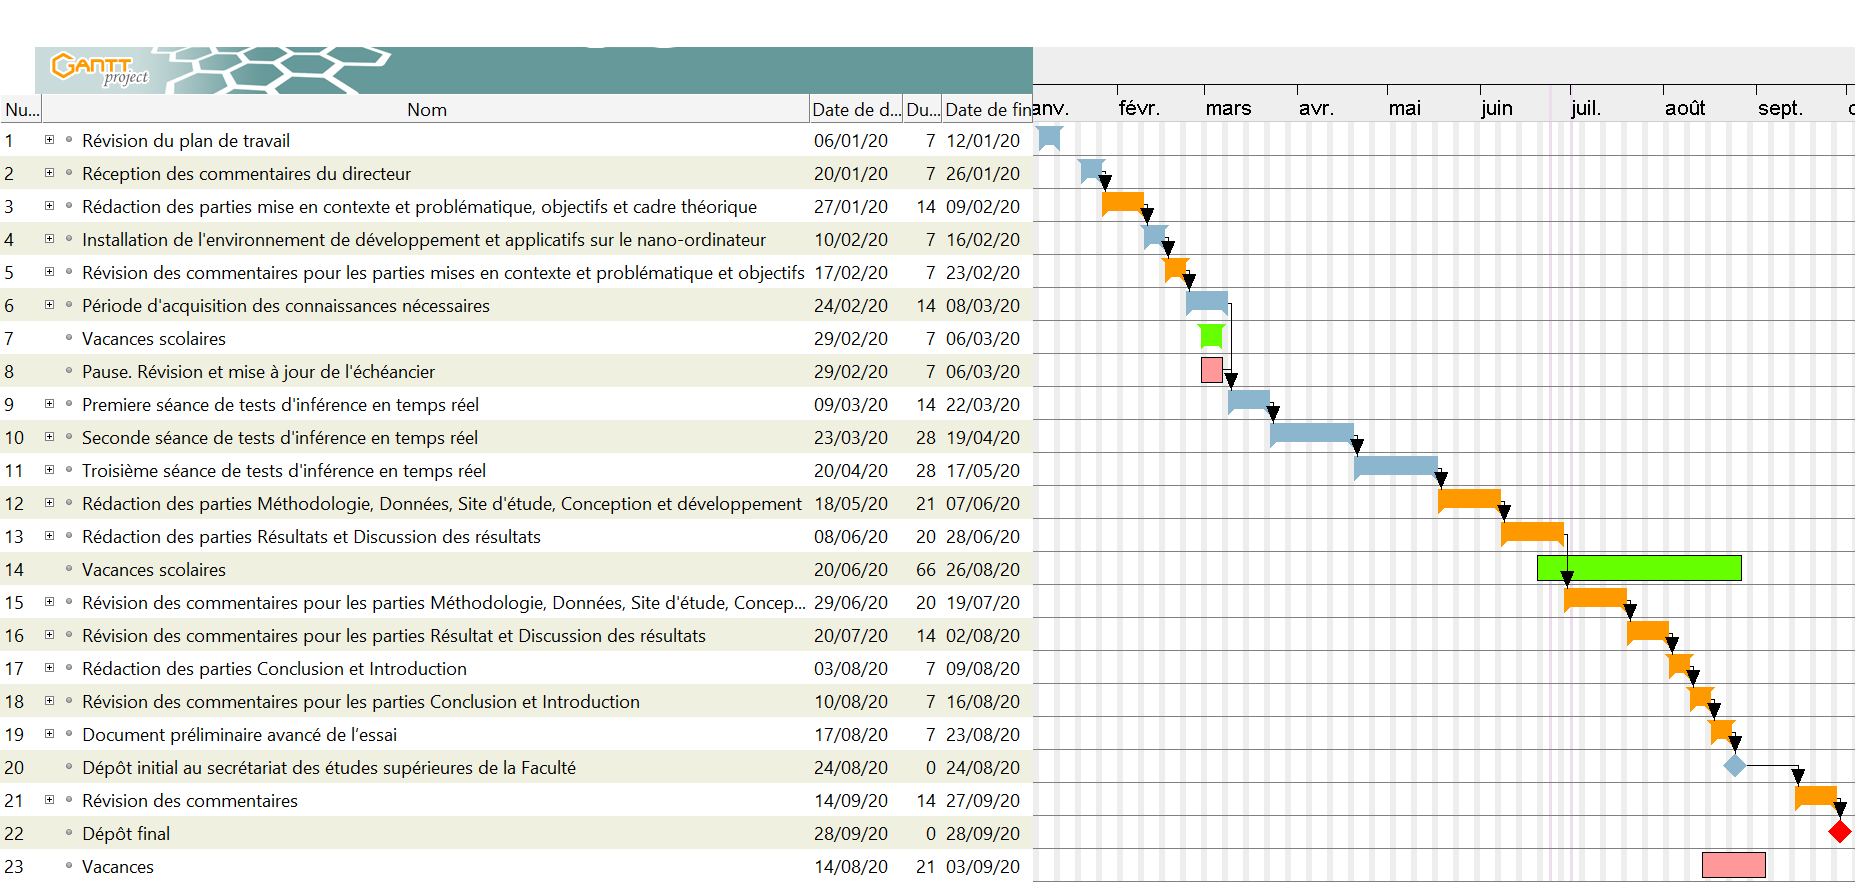
\includegraphics[width=1.4\textwidth, height=1.0\textheight]{echeancier}
      \caption{Échéancier}
      \label{fig:planning}
   \end{figure}
\end{landscape}

\clearpage 
\newpage
\printbibliography[title={\bibname\label{bib:references}}] 
\end{document}